\documentclass[a4paper,12pt]{article}
\usepackage[margin=1in]{geometry}
\usepackage [utf8]{inputenc}
\usepackage{moreverb}
\usepackage{listings}
\usepackage{graphicx}
\usepackage{verbatim}
\usepackage{amsmath}
\usepackage{amsfonts}
\usepackage{lastpage}
\usepackage{url}
\usepackage{minted}

\usemintedstyle{colorful}

\usepackage{fancyhdr}
\pagestyle{fancy}
\lhead{Multi-Paradigm Assignment\\ TIPLPA}
\chead{26-05-2014 \\}
\rhead{Lasse Brøsted Pedersen\\ 10769 - Group 4}
\lfoot{}
\cfoot{}
\rfoot{Page \thepage ~of \pageref{LastPage}}

\DeclareGraphicsExtensions{.pdf,.png,.jpg}

\newcommand{\code}[1]{{\fontfamily{pcr}\selectfont #1}}

\begin{document}

\section{Functionality of the Application}

\begin{figure}[h]
	\centering
	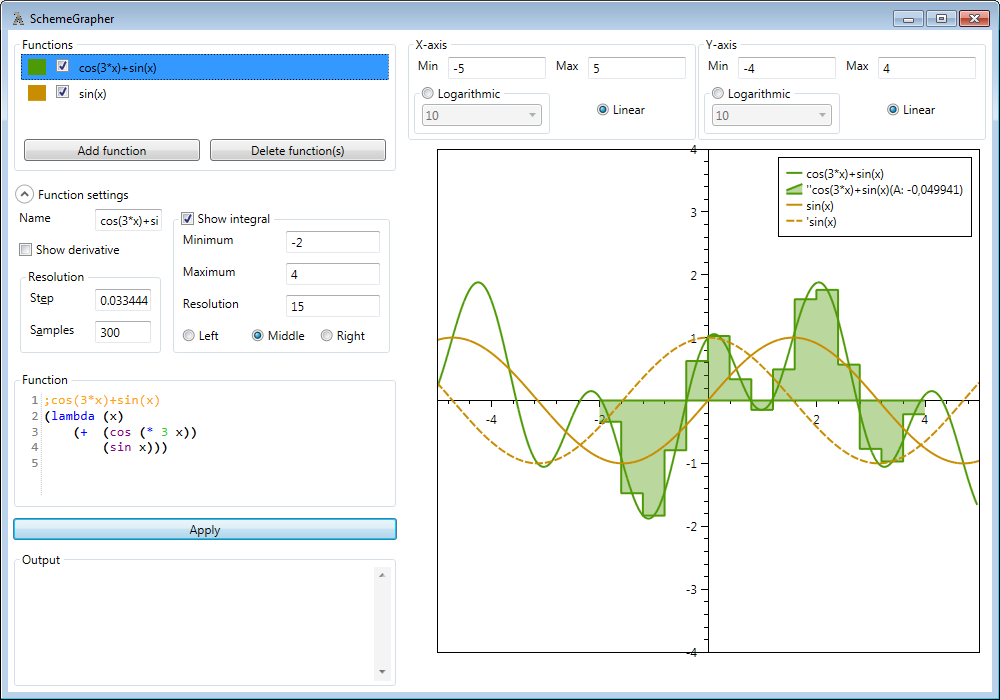
\includegraphics[scale=0.5]{schemegraphersscreen1}
	\caption{Screen dump showing various functionality of the application. }
    \label{fig:screendump}
\end{figure}

This window is split up in grids, whereas different options are customizable on how and which functions are to be shown as graphs in the Graph Section on the right side. First of all, a function is to be selected in the upper left corner. These functions are bound to their individual settings, which are shown below the function list in the ‘Function settings’ dropdown box. In the Function list, each function has a checkbox attached which indicates if the selected function is drawn in the Graph Section. The background color of the Function list items matches the respective graphs in the Graph Section to give a better overview of which functions matches which graphs. In addition to this, it is possible to add and remove functions from the list.

The settings of the functions are to be changed and set in the Function settings box. The step size and number of samples can be set to change the resolution of the graph. In addition to this, the derivative and integral can be shown, with additional settings on the integral on the resolution and the minimum and maximum values of the integral calculation. All these settings are only set for the current function selected in the Function list.

Below the settings box, the Function code box is shown. This box is an editable textbox where the code for the corresponding chosen list item in the Function list is shown. This code can be corrected and applied to the Graph Section by clicking the 'Apply' button below the box. 
The last box in the left side is the Output box. In this box all the output from the applied code is written. This box is also for error messages for syntactical errors and other exceptions.

The right side of the GUI is the Graph section. At the top, some settings are shown, specific to the Graph layout, that is, these functions are valid for all the functions where the left side options are specific for each of the functions. Here the minimum and maximum values of the X and Y axes can be changed, and also if the axes are to linear or logarithmic. Additional logarithmic settings are available for either $log_2$, $log_{10}$ or $ln$.
The rest of the GUI is the Graph, where the checked functions in the Function list are shown as well as their derivatives and integrals, if checked. The legend shows the functions names and colors. In addition, for the integrals shown, the result of the integral is shown in the legend of the integral.

\section{Architecture}

As required by the assignment, the application is split into two parts: all mathematical calculations are handled in Scheme -  GUI and control flow of the program is handled by the (mostly) imperative language C\#. For this project, the scheme implementation used is IronScheme\footnote{\url{http://ironscheme.codeplex.com/}} which is implemented on the .NET platform, and thus integrates well with C\# and vice versa. The layers of the application is shown in figure \ref{fig:layers}.

\begin{figure}[h]
	\centering
	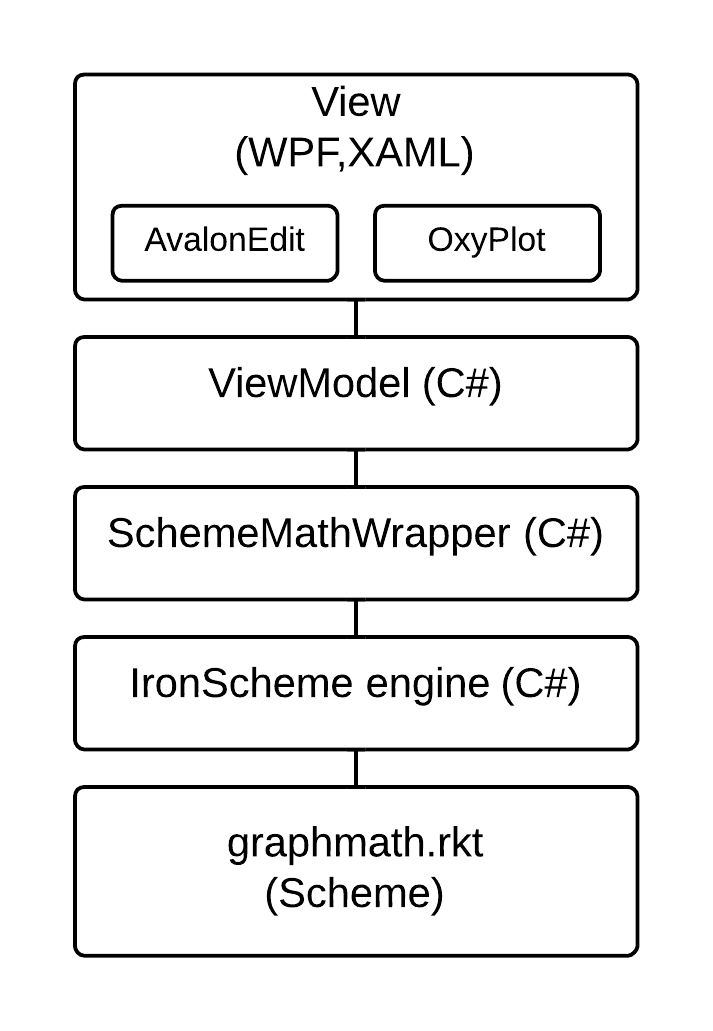
\includegraphics[scale=0.23]{MultiParadigmeBlocks}
	\caption{Layers of the application}
    \label{fig:layers}
\end{figure}

As figure \ref{fig:layers} shows, the application is based on .NET with a GUI written in WPF(Windows Presentation Foundation) using the Model-View-ViewModel(MVVM)-pattern. The view presents the graphical interface, and allows the user to interact with the application. AvalonEdit is a custom control for textediting that provides syntax highlighting, and OxyPlot is the charting control used. The viewmodel interacts with the model, the SchemeMathWrapper and presents data to the view.

\subsection{Bridging IronScheme and C\#}
 
The purpose of the SchemeMathWrapper is to provide the bridge between the imperative C\# application, and the functional Scheme procedures. Bridging involves translating from C\# function calls to Scheme procedure calls, and back and forth between native types of each paradigm.

\begin{listing}[H]
\begin{minted}[fontsize=\footnotesize, linenos]{csharp}
IEnumerable<Tuple<double, double>> CalcPlotData(string f, double min, double max, double step)
{
    var xyCons = "(calc-plot-data {0} {1} {2} {3})".Eval<Cons>(f.Eval(), min, max, step);

    //convert from Cons<Cons> (pseudo) to IEnumerable<Tuple<double, double>>
    return CreateListOfTuples(xyCons);
}
\end{minted}	

\caption{Bridging in \code{SchemeMathWrapper.CalcPlotData()}.}
\label{lst:SchemeCalcWrap}
\end{listing}

The C\# function in listing \ref{lst:SchemeCalcWrap} shows how bridging is done in the application. This particular function calculates the xy-coordinate pairs for the scheme procedure \code{f} passed as a string. The string \code{f} is evaluated to obtain a scheme procedure and passed to the evaluation of the scheme expression as argument \code{\{0\}}. Prior to using this function, the scheme procedure \code{calc-plot-data} has been loaded into the IronScheme engine by evaluating the contents of the file \code{schememath.rkt}, which contains regular scheme procedure definitions such as this one:

\begin{minted}[fontsize=\footnotesize]{scheme}
(define calc-plot-data
  (lambda (f min max step)
    ..
\end{minted}	

Evaluating the function returns a scheme list, represented as the C\# class \code{Cons} (part of IronScheme), where each \code{car} element is a \code{Cons}-pair containing a x and y value. Since IronScheme is based on .NET, it shares most data types (apart from \code{cons}) such as \code{string, int, double, array} and \code{Stream} with other .NET languages. IronScheme provides methods for converting back and forth between IronScheme procedures and .NET delegates allowing functions/procedures to be passed in both directions.
\\

The overall flow sequence of drawing a single function is a shown in figure \ref{fig:sequence}.

\begin{figure}[h]
	\centering
	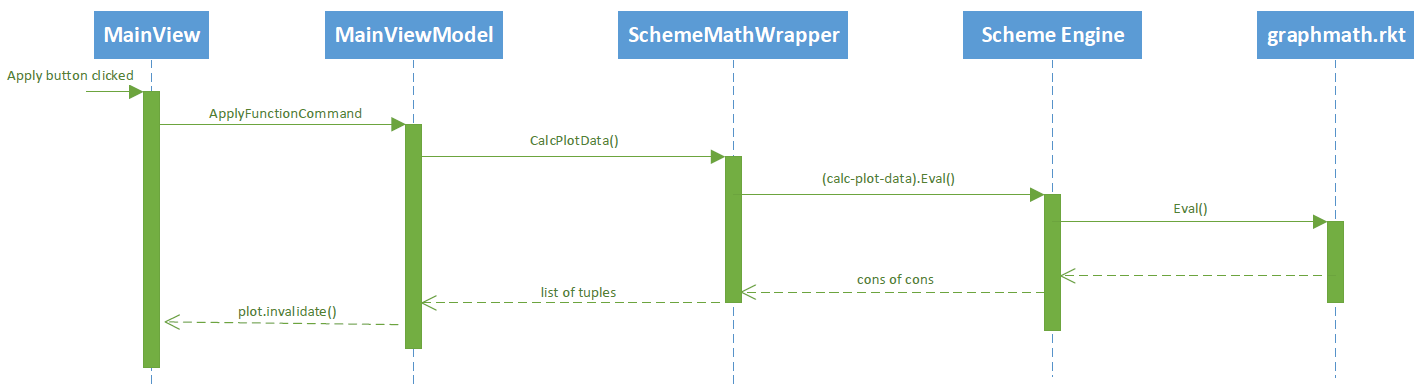
\includegraphics[scale=0.45]{sequence}
	\caption{Sequence diagram for calculating plot values (simplified)}
    \label{fig:sequence}
\end{figure} 



\begin{itemize}
\item validation close to model vs gui feedback
\end{itemize}
		
\section{Testing Strategy}	
The application was tested by two test suites. One test suite was a .NET test written i C\# using the built-in test framework MSTest, which tests the C\# portion of the application. The other test suite was a unit test written in Scheme to test the business logic (ie. mathematical calculations) used for this application. 

The scheme test is performed using the standalone IronScheme interpreter, so as to not introduce any errors that may be caused by hosting IronScheme in a C\# application. 
Although unit test frameworks are available for scheme, none were used for this project, as having a framework was not essential for showing testing for this small application.

\begin{listing}[H]
\begin{minted}{scheme}
(define test:calc-plot-data 
  (equal? (calc-plot-data f 0 2 1/2) expected-plot-data))
\end{minted}	

\caption{Scheme test of \code{calc-plot-data}.}
\label{lst:SchemeTest}
\end{listing}

The C\# portion tested was primarily the C\# wrapper for the IronScheme code, since that is the central part of this application. The role of this test suite is to verify that the bridge works as expected, ie. correct scheme procedures are called with the correct arguments and the conversion to and from the data types of each language works as expected. The test of the wrapper is tested using the same (or equivalent) input and expected output as the pure scheme test to ensure correct behaviour. This however, leads to extra testing, because the same procedure/function is tested twice.

\begin{listing}[H]
\begin{minted}{csharp}
[TestMethod]
public void calcPlotData()
{
    var actual = SchemeMathWrapper.CalcPlotData(f, 0, 2, 0.5).ToList();

    CollectionAssert.AreEqual(expectedPlotData, actual);
}
\end{minted}	

\caption{Test of C\# wrapper for \code{calc-plot-data}.}
\label{lst:SchemeTest}
\end{listing}

Other parts of the application, in particular the viewmodel and  the GraphFunction class representing a single function and related properties should also be tested. These have not been tested in this project, but can be tested in the same manner as the IronScheme wrapper. 

	
\end{document}